\documentclass[a4paper]{article}
\usepackage[UTF8]{ctex}
\usepackage{geometry}
\usepackage{graphicx}
\usepackage{url}
\usepackage{multirow}
\usepackage{array}
\usepackage{booktabs}
\usepackage{url}
\usepackage{enumitem}
\usepackage{graphicx}
\usepackage{float}
\usepackage{amssymb}
\usepackage{amsmath}
\usepackage{subfig}
\usepackage{longtable}

\geometry{a4paper, scale=0.78}
\title{ Math Basis}
\author{罗文水}

% 公式标号跟章节关联
\numberwithin{equation}{section}

\begin{document}
\maketitle
\tableofcontents

\newpage
\section{Math Basis 01}

本节的主要目的是从频率派的角度使用极大似然估计,通过观察到数据,是观察到的数据出现的概率最大化,来对高斯分布的参数进行估计。并且分析了高斯分布的参数,$\mu$,$\sigma^2$的无偏性和有偏性。其中,$\mu$是关于参数的无偏估计,而$\sigma$是有偏估计。

数据矩阵为:

\begin{equation}
    X=(x_1, x_2, \cdots, x_N)^T=
    \begin{pmatrix}
    x_1^T \\ 
    x_2^T \\
    \vdots\\
    x_N^T \\
    \end{pmatrix} =
    \begin{pmatrix}
    x_{11} & x_{12} & \dots & x_{1p}\\
    x_{21} & x_{32} & \dots & x_{2p}\\
    \vdots & \vdots & \ddots & \vdots\\
    x_{N1} & x_{N2} & \dots & x_{Np}\\
    \end{pmatrix}_{N\times p}
\end{equation}

在数据矩阵的基础上,有$x_i \in \mathbb{R}$,$x_i \sim \mathcal{N}(\mu, \Sigma)$,那么参数为$\theta=\mu, \Sigma$。

\subsection{求解目的}
首先对于单变量的高斯分布$\mathcal{N}(\mu,\sigma^2)$,概率密度函数为:
\begin{equation}
    p(x)=\frac{1}{\sqrt{2\pi}\sigma}exp\left\{ -\frac{(x-\mu)^2}{2\sigma^2} \right\}
\end{equation}

对于多变量的高斯分布$\mathcal{N}(\mu,\Sigma)$,概率密度函数为:
\begin{equation}
    p(x)=\frac{1}{(2\pi)^{\frac{p}{2}}|\Sigma|^{\frac{1}{2}}}exp\left\{ -\frac{1}{2}(x-\mu)^T\Sigma^{-1}(x-\mu) \right\}
\end{equation}

我们希望通过观察到的数据来计算参数$\theta=(\mu,\Sigma)$的值,那么我们使用极大似然估计的优化目标为$\theta_{MLE}=\arg\max_{\theta}p(X|\theta)$。于是我们可以转化为$\theta_{MLE}=\arg\max_{\theta}\log p(X|\theta)$。那么,计算公式可以化简为:
\begin{align}
    \arg\max_{\theta}\log p(X|\theta) = & \log \prod_{i=1}^N p(x_i|\theta)=\sum_{i=1}^N \log p(x_i|\theta) \\
    = & \sum_{i=1}^N \left(\log \frac{1}{\sqrt{2\pi}} + \log \frac{1}{\sigma} - \frac{(x-\mu)^2}{2\sigma^2} \right)
\end{align}

\subsection{极大似然法求解参数$\mu$和$\sigma^2$}
在求解$\mu_{MLE}$时,计算目标为$\frac{\partial\log p(x|\theta)}{\partial \mu}$,推导公式如下:
\begin{align}
    \frac{\partial\log p(x|\theta)}{\partial \mu} = & \sum_{i=1}^N - \frac{(x_i-\mu)}{\sigma^2} = 0
\end{align}
\begin{gather}
    \sum_{i=1}^N x_i =  \sum_{i=1}^N \mu \\
    \mu_{MLE} =  \frac{1}{N}\sum_{i=1}^N x_i
\end{gather}

在求解$\sigma^2_{MLE}$时,计算目标为$\frac{\partial\log p(x|\theta)}{\partial \sigma}$,推导公式如下:
\begin{gather}
    \frac{\partial\log p(x|\theta)}{\partial \sigma} 
     = \sum_{i=1}^N - \frac{1}{\sigma} - \frac{1}{2}(x_i-\mu)^2(-2)\sigma^{-3} = 0 \\
     \sum_{i=1}^N  \sigma^2 = \sum_{i=1}^N (x_i-\mu)^2 \\
     \sigma^2_{MLE} = \frac{1}{N} \sum_{i=1}^N (x_i-\mu)^2 
\end{gather}

实际上这里的$\mu$是$\mu_{MLE}$,所以,
\begin{equation}
    \sigma^2_{MLE} = \frac{1}{N} \sum_{i=1}^N (x_i-\mu_{MLE})^2 
\end{equation}

\subsection{验证$\mu_{MLE}$和$\sigma^2_{MLE}$的无偏性}
首先需要明确什么是无偏估计,所谓无偏估计也就是,$\mathbb{E}(\hat{x})=x$。那么利用这个性质我们就可以很方便的判断一个估计是否为无偏估计。
\subsubsection{验证$\mu_{MLE}$的无偏性}

\begin{equation}
    \begin{split}
        \mathbb{E}[\mu_{MLE}] = & \mathbb{E}[\frac{1}{N} \sum_{i=1}^N x_i] \\
        = & \frac{1}{N} \sum_{i=1}^N \mathbb{E}[  x_i] \\
        = & \frac{1}{N} N \mu = \mu
    \end{split}
\end{equation}


根据上述的推导,我们可以得出$\mu_{MLE}$是无偏估计。

\subsubsection{验证$\sigma^2_{MLE}$的无偏性}

\begin{equation}
    \begin{split}
        \mathbb{E}[\sigma^2_{MLE}] = & \mathbb{E}[ \frac{1}{N}\sum_{i=1}^N (x_i-\mu_{MLE})^2] \\
        = & \mathbb{E}[ \frac{1}{N}\sum_{i=1}^N (x_i^2-2\mu_{MLE} x_i + \mu_{MLE}^2)] \\
        = & \mathbb{E}[ \frac{1}{N}\sum_{i=1}^N (x_i^2- \mu_{MLE}^2)]\\
        = & \mathbb{E}[ \frac{1}{N}\sum_{i=1}^N (x_i^2-\mu^2)-(\mu_{MLE}^2-\mu^2)] \\
        = & \mathbb{E}[ \frac{1}{N}\sum_{i=1}^N (x_i^2-\mu^2)]-\mathbb{E}[(\mu_{MLE}^2-\mu^2)]\\
        = & \mathbb{E}[ \frac{1}{N}\sum_{i=1}^N (x_i^2-(\frac{1}{N}\sum_{i=1}^Nx_i)^2)]-\mathbb{E}[(\mu_{MLE}^2-\mu^2)]\\
        = & \frac{1}{N}\sum_{i=1}^{N}(\mathbb{E}[x_i^2]-\mathbb{E}[x]^2)-\mathbb{E}[(\mu_{MLE}^2-\mu^2)] \\
        = & \sigma^2 - (\mathbb{E}[\mu_{MLE}^2] - \mathbb{E}[\mu^2]) \\
        = & \sigma^2 - (\mathbb{E}[\mu_{MLE}^2] - \mathbb{E}[\mathbb{E}[\mu_{MLE}]^2]) \\
        = & \sigma^2 - (\mathbb{E}[\mu_{MLE}^2] - \mathbb{E}[\mu_{MLE}]^2] \\
        = & \sigma^2 - Var[\mu_{MLE}] \\
        = & \sigma^2 - Var[\frac{1}{N}\sum_{i=1}^Nx_i] \\
        = & \sigma^2 - \frac{1}{N^2}Var[\sum_{i=1}^Nx_i] \\
        = & \sigma^2 - \frac{1}{N^2}\sum_{i=1}^NVar[x_i] \\ 
        = & \sigma^2 - \frac{1}{N^2} N \sigma^2 \\
        = & \frac{N-1}{N}\sigma^2
    \end{split}
\end{equation}

有上述推导我们可以得出,$\sigma^2_{MLE}$为有偏估计量,而且和真实值比较偏小。为什么会造成这个结果呢?主要原因是出在$\mu_{MLE}$上,因为我们在求$\sigma^2_{MLE}$时使用的是$\mu_{MLE}$而不是$\mu$。而$\mu_{MLE}$是拟合数据得到的,所以波动的角度讲,肯定会比使用真实的$\mu$算出来要小。所以在高斯分布中,利用极大似然估计得到的$\sigma^2_{MLE}$的值,是比真实值偏小的有偏估计。

\section{Math Basis 02 }

本节的主要目的是从概率的角度来分析高斯分布,包括马氏距离和高斯分布的几何表示,以及高斯分布的局限性和解决的方法等等。对于多变量的高斯分布$X\sim \mathcal{N}(\mu,\Sigma)$,概率密度函数为:
\begin{equation}
    p(x)=\frac{1}{(2\pi)^{\frac{p}{2}}|\Sigma|^{\frac{1}{2}}}exp\left\{ -\frac{1}{2}(x-\mu)^T\Sigma^{-1}(x-\mu) \right\}
\end{equation}
其中,$x\in\mathbb{R}^p$,
\begin{equation}
    x=
    \begin{pmatrix}
        x_1 \\
        x_2 \\
        \vdots \\
        x_p
    \end{pmatrix} \qquad \qquad
    \Sigma = 
    \begin{pmatrix}
        \sigma_{11} & \sigma_{12} & \cdots & \sigma_{1p} \\
        \sigma_{21} & \sigma_{22} & \cdots & \sigma_{2p} \\
        \vdots      & \vdots      & \ddots & \vdots      \\
        \sigma_{p1} & \sigma_{p2} & \cdots & \sigma_{pp}
        \end{pmatrix}
\end{equation}
其中,$\Sigma$为正定矩阵或者半正定矩阵。

\subsection{什么是马氏距离}
在高斯分布中,$\sqrt{(x-\mu)^T\Sigma^{-1}(x-\mu)}$的计算结果是一个数,这个数被称为马氏距离。设$z_1=(z_{11}, z_{12})^T$,$z_2=(z_{21}, z_{22})^T$。那么$z_1$和$z_2$之间的马氏距离的平方为:
\begin{equation}
    (z_1-z_2)^T\Sigma^{-1}(z_1-z_2)=
    \begin{pmatrix}
        z_{11}-z_{12} & z_{21}-z_{22}
    \end{pmatrix}
    \Sigma^{-1}
    \begin{pmatrix}
        z_{11}-z_{12} \\
        z_{21}-z_{22}
    \end{pmatrix}
\end{equation}

显然,当$\Sigma^{-1}=I$时,马氏距离等于欧式距离$ (z_1-z_2)^T\Sigma^{-1}(z_1-z_2)=(z_{11}-z_{12})^2+(z_{21}-z_{22})^2$。

\subsection{对$(x-\mu)^T\Sigma^{-1}(x-\mu)$的值进行推导}
由于$\Sigma$为实对称矩阵,那么可以对$\Sigma$进行特征分解,那么有$\Sigma = U\Lambda U^T$,并且$UU^T=U^TU=I$,所以$U^{-1}=U^T$,$\Lambda=diag(\lambda_i)\quad(i=1,2,\cdots,N)$,并且$U=(u_1,u_2,\cdots,u_p)_{p\times p}$。

\begin{align}
    \Sigma = & U\Lambda U^T \\
    = & (u_1,u_2,\cdots,u_p)
    \begin{pmatrix}
        \lambda_1 & & & \\
        & \lambda_2 & & \\
        & & \ddots & \\
        & & & \lambda_p \\
    \end{pmatrix}
    \begin{pmatrix}
        u_1^T  \\
        u_2^T  \\
        \vdots \\
        u_p^T  \\
    \end{pmatrix} \\
     = & (u_1\lambda_1,u_2\lambda_2,\cdots,u_p\lambda_p)
     \begin{pmatrix}
        u_1^T  \\
        u_2^T  \\
        \vdots \\
        u_p^T  \\
    \end{pmatrix} \\
    = & \sum_{i=1}^{p}u_i\lambda_i u_i^T
\end{align}

而$\Sigma^{-1}$的求解过程如下所示:

\begin{equation}
    \Sigma^{-1} = (U \Lambda U^T)^{-1} = (U^T)^{-1} \Lambda^{-1} U^{-1} = U \Lambda^{-1} U^T
\end{equation}

代入可以解得:
\begin{equation}
    \Sigma^{-1} = \sum_{i=1}^{p}u_i\frac{1}{\lambda_i} u_i^T
\end{equation}

那么,
\begin{align}
    (x-\mu)^T\Sigma^{-1}(x-\mu) = & (x-\mu)^T\sum_{i=1}^{p}u_i\frac{1}{\lambda_i} u_i^T(x-\mu) \\
    = & \sum_{i=1}^{p} (x-\mu)^Tu_i\frac{1}{\lambda_i} u_i^T(x-\mu)
\end{align}

令$y_i=(x-\mu)^Tu_i$,这是一个典型的投影算法,其中$u_i$是$\Sigma$的特征值为$\lambda_i$的特征向量,那么
\begin{equation}
    (x-\mu)^T\Sigma^{-1}(x-\mu) = \sum_{i=1}^{p} y_i\frac{1}{\lambda_i} y_i^T=\sum_{i=1}^p\frac{y_i^2}{\lambda_i}
\end{equation}

\subsection{高斯分布的几何意义}
如何令$p=2$,则有$\Delta = \frac{y_1^2}{\lambda_1} + \frac{y_2^2}{\lambda_2} $,这实际上就是一个椭圆,如果$\Delta$取不同的值,就会像等高线一样,一圈圈的环绕,因为每一个$\Delta$都对应着一个二次型,即对应着概率密度函数的一个取值,同样的$\Delta$取值对应着同样的概率密度。那么最终的概率密度等高线表示为:
\begin{figure}[H]
    \centering
    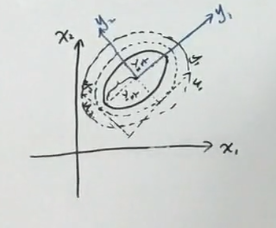
\includegraphics[width=.5\textwidth]{20191019203302.png}
    \caption{二维高斯分布的可视化表示图}
    \label{fig:my_label_1}
\end{figure}


\subsection{高斯分布中遇到的困难}
\subsubsection{维度灾难(curse of dimension)}
由于$\Sigma$是一个$p\times p$的矩阵,矩阵中一共有$\frac{p(p+1)}{2}$个参数,算法的复杂度为$O(p^2)$。一旦输入维度过大,这个矩阵的计算会变得很复杂。所以,在某些时候,将$\Sigma$矩阵简化成对角矩阵将算法复杂度降低到$O(p)$。进一步简化,可以令$\lambda_1=\lambda_2=\cdots=\lambda_p$。这时,高斯分布的可视化表示即为一个中心在原点的同心圆。这样的高斯分布,被我们称为“各向同性”的高斯分布。

\subsubsection{高斯分布的表达的局限性}
很多时候,高斯分布的表达有局限性,这时,学者提出了混合高斯模型(GMM)来拟合现实情况中复杂多样的分布。具体有关于混合高斯模型(GMM)的内容将在后续部分进行详细解释,


\section{Math Basis 03 }
本节的主要内容是在高斯分布中,已知联合概率密度求条件概率密度和边缘概率密度。还有已知$x$的边缘概率和在条件为$x$下$y$的条件概率下,求$y$的边缘概率和在条件为$y$下$x$的条件概率。用数学的语言描述即为,如下所示。

对于多变量的高斯分布$x\sim \mathcal{N}(\mu,\Sigma)$,概率密度函数为:
\begin{equation}
    p(x)=\frac{1}{(2\pi)^{\frac{p}{2}}|\Sigma|^{\frac{1}{2}}}exp\left\{ -\frac{1}{2}(x-\mu)^T\Sigma^{-1}(x-\mu) \right\}
\end{equation}
其中,$x\in\mathbb{R}^p$,
\begin{equation}
    x=
    \begin{pmatrix}
        x_1 \\
        x_2 \\
        \vdots \\
        x_p
    \end{pmatrix} \qquad \qquad
    \Sigma = 
    \begin{pmatrix}
        \sigma_{11} & \sigma_{12} & \cdots & \sigma_{1p} \\
        \sigma_{21} & \sigma_{22} & \cdots & \sigma_{2p} \\
        \vdots      & \vdots      & \ddots & \vdots      \\
        \sigma_{p1} & \sigma_{p2} & \cdots & \sigma_{pp}
        \end{pmatrix}_{p\times p}
\end{equation}

已知联合概率密度求条件概率密度和边缘概率密度,可描述为已知:
\begin{equation}
    x= 
    \begin{pmatrix}
        x_a \\
        x_b
    \end{pmatrix}
    \quad m+n=p \quad
    \mu=
    \begin{pmatrix}
        \mu_a \\
        \mu_b
    \end{pmatrix} \quad
    \Sigma=
    \begin{pmatrix}
    \Sigma_{aa} & \Sigma_{ab} \\
    \Sigma_{ba} & \Sigma_{bb} 
    \end{pmatrix}
\end{equation}

求:$p(x_a)$和$p(x_b|x_a)$

另一个可描述为,已知:
$p(x)=\mathcal{N}(x|\mu,\Lambda^{-1})$,$p(y|x)=\mathcal{N}(Ax+b,L^{-1})$,求$p(y)$和$p(x|y)$。

\subsection{已知联合概率密度求条件概率密度和边缘概率密度}
在进行此次推导之前,首先需要引入一个推论。已知:
\begin{gather}
    x\sim \mathcal{N}(\mu,\Sigma) \\
    y = Ax + b
\end{gather}

那么可以解得:$y\sim \mathcal{N}(A\mu+b, A\Sigma A^T)$。
\subsubsection{求解边缘概率密度$p(x_a)$}
\begin{equation}
    x_a = (I_m,0)
    \begin{pmatrix}
        x_a \\
        x_b
    \end{pmatrix}
\end{equation}

很显然,等式的第一部分就是$A$,等式的第二部分就是$X$,那么
\begin{equation}
    \begin{split}
        \mathbb{E}[x_a]=(I_m,0)
    \begin{pmatrix}
        \mu_a \\
        \mu_b
    \end{pmatrix}
    \end{split}=\mu_a \qquad
    Var[x_a] = (I_m,0)
    \begin{pmatrix}
    \Sigma_{aa} & \Sigma_{ab} \\
    \Sigma_{ba} & \Sigma_{bb} 
    \end{pmatrix}
    \begin{pmatrix}
    I_m \\
    0  
    \end{pmatrix}=\Sigma_{aa}
\end{equation}

所以,$x_a\sim \mathcal{N}(\mu_a, \Sigma_{aa})$,同理$x_b \sim \mathcal{N}(\mu_b,\Sigma_{bb})$。

\subsubsection{求解条件概率密度$p(x_b|x_a)$}
这里使用的是构造证明法,有一点猜出了结论,再使用结论来证结论的感觉。在这里引入了一个构造函数$x_{b\cdot a}=x_b-\Sigma_{ba}\Sigma_{aa}^{-1}x_a$。那么根据我们的推论,我们可以很简单的得出以下的构造方法
\begin{gather}
    \mu_{b\cdot a}= \mu_b-\Sigma_{ba}\Sigma_{aa}^{-1}\mu_a \\
    \Sigma_{bb \cdot a} = \Sigma_{bb}-\Sigma_{ba}\Sigma_{aa}^{-1}\Sigma_{ab} 
\end{gather}

其中$\Sigma_{aa\cdot b}$被称为$\Sigma_{aa}$的Schur Complementary。我们接下来可以很简单的将$x_{b\cdot a}$化简成$Ax+b$的性质。
\begin{equation}
    x_{b\cdot a} = (-\Sigma_{ba}\Sigma_{aa}^{-1}\quad I_m)
    \begin{pmatrix}
        x_a \\
        x_b
    \end{pmatrix}
\end{equation}

那么我们进行以下的推导,
\begin{equation}
    \mathbb{E}[x_{b\cdot a}]= (-\Sigma_{ba}\Sigma_{aa}^{-1}\quad I_m)
    \begin{pmatrix}
        \mu_a \\
        \mu_b
    \end{pmatrix}
    =\mu_b-\Sigma_{ba}\Sigma_{aa}^{-1}\mu_a
\end{equation}
\begin{equation}
    Var[x_{b\cdot a}]=(-\Sigma_{ba}\Sigma_{aa}^{-1}\quad I_m)
    \begin{pmatrix}
    \Sigma_{aa} & \Sigma_{ab} \\
    \Sigma_{ba} & \Sigma_{bb} 
    \end{pmatrix}
    \begin{pmatrix}
        -{\Sigma_{aa}^{-1}}^T \Sigma_{ba}^T \\
        I_m
    \end{pmatrix}
\end{equation}

计算得出,$Var[x_{b\cdot a}]=\Sigma_{bb}-\Sigma_{ba}\Sigma_{aa}^{-1}\Sigma_{ab} $。所以,$p(x_{b\cdot a})=\mathcal{N}(\mu_{b\cdot a},\Sigma_{bb\cdot a})$。

又因为$x_b=x_{b\cdot a}+\Sigma_{ba}\Sigma_{aa}^{-1}x_a$,$x_b$是一个关于$x_a$的线性表达。那么后续的求解过程将变得非常的简单了。
\begin{equation}
    \mathbb{E}[x_b|x_a]=\mathbb{E}[x_{b\cdot a}] + \Sigma_{ba}\Sigma_{aa}^{-1}x_a = \mu_b+\Sigma_{ba}\Sigma_{aa}^{-1}(x_a-\mu_a)
\end{equation}

而$Var[x_b|x_a]$中
\begin{equation}
    Var[x_b|x_a] = \Sigma_{bb \cdot a} = \Sigma_{bb}-\Sigma_{ba}\Sigma_{aa}^{-1}\Sigma_{ab}
\end{equation}

于是综上所述,$x_b|x_a\sim \mathcal{N}(\mu_b+\Sigma_{ba}\Sigma_{aa}^{-1}(x_a-\mu_a), \Sigma_{bb}-\Sigma_{ba}\Sigma_{aa}^{-1}\Sigma_{ab})$。

同理可得$x_a|x_b\sim \mathcal{N}(\mu_a+\Sigma_{ab}\Sigma_{bb}^{-1}(x_b-\mu_b), \Sigma_{aa}-\Sigma_{ab}\Sigma_{bb}^{-1}\Sigma_{ba})$。

\subsection{边缘高斯和条件高斯}
问题可以被描述为,$p(x)=\mathcal{N}(x|\mu,\Lambda^{-1})$,$p(y|x)=\mathcal{N}(Ax+b,L^{-1})$,求$p(y)$和$p(x|y)$。

这个高斯分布的公式的推导非常的重要,特别是在Linear Gaussian Model中被大量的运用。同时也在贝叶斯公式中有着大量的运用,所以某种意义上说,这个公式的运用比上一个公式更加的重要。

\subsubsection{边缘高斯}

根据已知条件,我们可以设$y=Ax+b+\varepsilon$,其中$\varepsilon\sim\mathcal{N}(0,L^{-1})$。
\begin{equation}
    \mathbb{E}[y]=\mathbb{E}[Ax+b+\varepsilon] = \mathbb{E}[Ax+b]+ \mathbb{E}[\varepsilon] = A\mu +b
\end{equation}
\begin{equation}
    Var[y] = Var[Ax+b+\varepsilon] = Var[Ax]+Var[\varepsilon]=A\Lambda^{-1}A^T +L^{-1}
\end{equation}

所以综上所述,$p(y)\sim\mathcal{N}(A\mu +b, A\Lambda^{-1}A^T +L^{-1})$。

\subsubsection{条件高斯}
根据上述的推导我们已经知道的条件有,$p(y)$,$p(x)$,$p(y|x)$那么我们可以如何求得$p(x|y)$呢?很显然我们还差一个$x$和$y$的联合分布。如果知道$x$和$y$的联合分布,那么我们就和上一节已知联合概率密度求条件概率密度和边缘概率密度的内容接起来了。

设
\begin{equation}
    z=
    \begin{pmatrix}
        x \\ 
        y
    \end{pmatrix} \sim
    \mathcal{N}
    \left(
    \begin{pmatrix}
        \mu \\
        A\mu + b \\
    \end{pmatrix}
    \quad
    \begin{pmatrix}
        \Lambda^{-1} & \Delta \\
        \Delta^T   & A\Lambda^{-1}A^T +L^{-1} \\
    \end{pmatrix}
    \right)
\end{equation}

这里的$\Delta$是$x$和$y$的协方差矩阵,我们可以直接利用协方差的定义来进行求解。
\begin{equation}
    \begin{split}
       \Delta = & Cov(x,y)= \mathbb{E}[(x-\mathbb{E}[x])(y-\mathbb{E}[y])^T]  \\
       = & \mathbb{E}[(x-\mu)(y-(A\mu + b))^T] \\
       = & \mathbb{E}[(x-\mu)(Ax+\varepsilon-A\mu)^T] \\
       = & \mathbb{E}[(x-\mu)(Ax-A\mu+\varepsilon)^T] \\
       = & \mathbb{E}[(x-\mu)(Ax-A\mu)^T+((x-\mu)\varepsilon)^T] \\
       = & \mathbb{E}[(x-\mu)(Ax-A\mu)^T]+\mathbb{E}[(x-\mu)\varepsilon^T] \\
  \end{split}
\end{equation}

$\mathbb{E}[(x-\mu)\varepsilon^T]=\mathbb{E}[(x-\mu)]\mathbb{E[\varepsilon^T]}=0$。那么,推导继续:
\begin{equation}
    \begin{split}
       \Delta
       = & \mathbb{E}[(x-\mu)(Ax-A\mu)^T] \\
       = & \mathbb{E}[(x-\mu)(x-\mu)^T]\cdot A^T \\
       = & Var[x]\cdot A^T \\
       = & \Lambda^{-1} A^T
  \end{split}
\end{equation}

所以,$x$和$y$之间的联合概率分布可表达为,
\begin{equation}
    z=
    \begin{pmatrix}
        x \\ 
        y
    \end{pmatrix} \sim
    \mathcal{N}
    \left(
    \begin{pmatrix}
        \mu \\
        A\mu + b \\
    \end{pmatrix}
    ,
    \begin{pmatrix}
        \Lambda^{-1} & \Lambda^{-1} A^T \\
        A\Lambda^{-1}  & A\Lambda^{-1}A^T +L^{-1} \\
    \end{pmatrix}
    \right)
\end{equation}

通过上述的推导,我们可以成功的得到$x$和$y$的联合概率密度分布。那么利用上节得出的公式,就可以成功的推导出$p(x|y)$。代入上述公式中,描述的结果如下:
\begin{equation}
    x|y\sim \mathcal{N}\left(\mu+\Lambda^{-1}A^TK^{-1}A\Lambda^{-1}\left(y-A\mu-b\right), \Lambda^{-1}-\Lambda^{-1}A^TK^{-1}A\Lambda^{-1}\right)
\end{equation}

其中,
\begin{equation}
    K=A\Lambda^{-1}A^T+L^{-1}
\end{equation}

\section{Math Basis 04}
本节主要的内容是描述琴生不等式(Jensen's Inequality)。有关琴生不等式的描述为,如果函数$f(x)$为凸函数(convex function),那么有$\mathbb{E}[f(x)]\geq f(\mathbb{E}[x])$。

\subsection{Jensen's Inequality中的证明}
\begin{figure}[H]
    \centering
    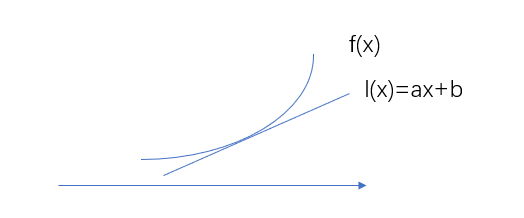
\includegraphics[width=.5\textwidth]{微信图片_20191021084621.png}
    \caption{函数和它在某点的切线的表达式}
\end{figure}

设切点的横坐标为$\mathbb{E}[x]$,那么$f(\mathbb{E}[x])=L(x)=a\mathbb{E}[x]+b$。又因为function为convex function。那么很显然,对于$\forall x$都有$f(x)\geq L(x)$。然后,我们同时对不等式两边求期望,可以得到$\mathbb{E}[f(x)]\geq \mathbb{E}[L(x)]$。那么我们进行如下的推导:
\begin{equation}
    \begin{split}
        \mathbb{E}[f(x)]\geq & \mathbb{E}[L(x)] \\
        = & \mathbb{E}[a\mathbb{E}[x]+b] \\
        = & a\mathbb{E}[x] + b \\
        = & f(\mathbb{E}[x]) \\
    \end{split}
\end{equation}
可以很简单的得出结论。

\end{document}
